
\input{example_proposal.bbl}
\clearpage


\appendix
\begin{deluxetable}{ccccccccc}
\tabletypesize{\scriptsize}

\tablecaption{DADOS Spectrograph Observations Log Sheet}
\tablewidth{0pt}
\tablehead{
\colhead{File} & \colhead{Object} &\colhead{Exp. Time (s)} & \colhead{Position
in the Slit}  & \colhead{Slit ($\mu
m$)} 
}
\startdata                                                                      
          
 cal/1 & Neon	&1	& in all of them	& 200		\\
cal/2 & Star - Altair	& 30	& middle	& 200		\\
cal/3 & Star - Altair	& 30	& bottom	& 200		\\
cal/4 & Star - Altair	& 60	& top	& 200		\\
bright/15/1-5& Moonshine	& 15
& Sky on top & 200	\\
bright/30/1-5& Moonshine	& 30
& Sky on top & 200	\\
dark/1-10& Earthshine	& 120	& Sky
on bottom & 200	\\
\enddata
\label{looo}
\end{deluxetable}


\begin{figure}[htb]
\begin{center}
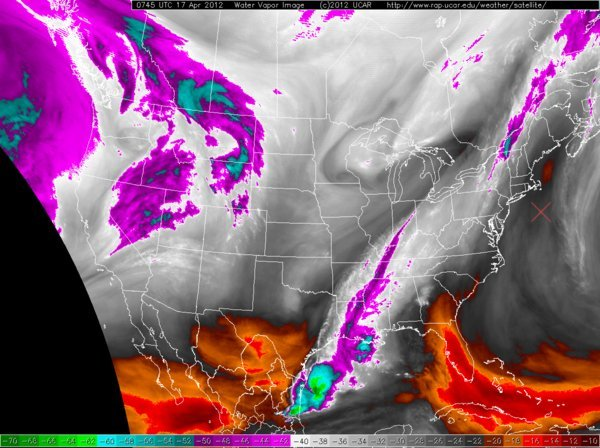
\includegraphics[scale=0.42]{figs/satt.jpg}
\caption{Cloud coverage on Earth for the period of observations.}
\label{sat}
\end{center}
\end{figure}

\begin{figure}[htb]
\begin{center}
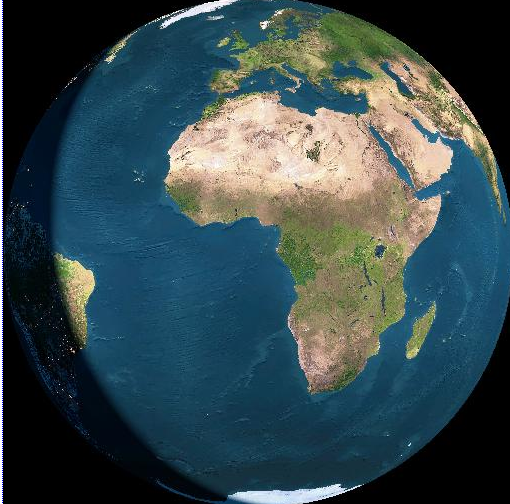
\includegraphics[scale=0.3]{figs/frommoon1.png}
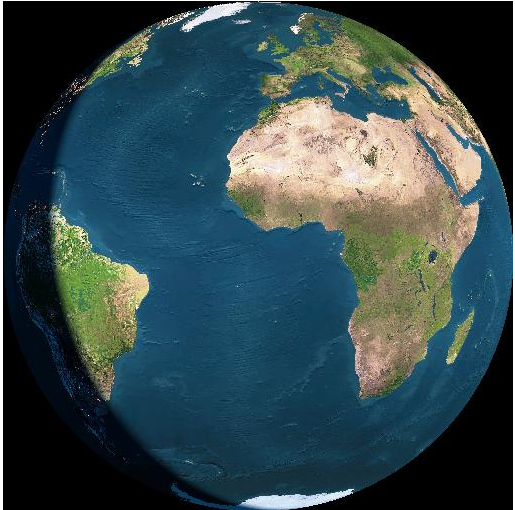
\includegraphics[scale=0.3]{figs/frommoon2.png}
\caption{Earth seen from the Moon in the begin and the end time of our
observations.}
\label{frommoon}
\end{center}
\end{figure}


\begin{figure}[htb]
\begin{center}
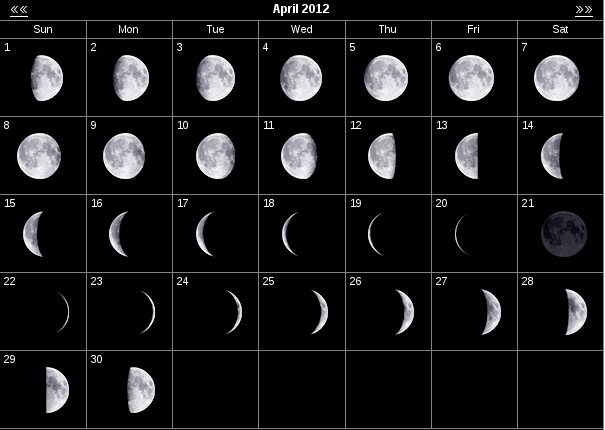
\includegraphics[scale=0.6]{figs/moon.png}
\caption{Phases of the moon for the month we were observing. The data was
taken on the 17th, a waning crescent moon.}
\label{moooon}
\end{center}
\end{figure}




